\documentclass[12pt]{article}

\usepackage{graphicx}
\usepackage{float}
\usepackage{setspace}
\usepackage{ulem}

\begin{document}

\title{EVIL Sparc Compiler}

\author{
By Christopher Hoover and Marc Zych \vspace{10pt} \\
CSC 520: Grad Computer Architecture \vspace{10pt} \\
Dr. Chris Lupo \vspace{10pt} \\
}
\date{June 4, 2012}

\maketitle

\vfill

\thispagestyle{empty}
\newpage

\tableofcontents
\newpage

\section{Introduction}
Our project involved implementing various compiler optimizations to determine their effects on program performance.
Instead of designing and implementing an entirely new compiler, we decided to modify an existing compiler designed for the SPARC architecture.
This allowed us to focus our efforts purely on optimizations.

The remainder of the paper is structured as follows.
Section 2 provides background information about the SPARC architecture.
Section 3 describes the initial state of the compiler before we performed our optimizations.
Section 4 describes each of the optimizations we performed.
Section 5 presents our results and Section 6 concludes.

\section{Background on the SPARC Architecture}
The SPARC architecture has 4 distinct types of registers: LOCAL, IN, OUT, and GLOBAL.
The LOCAL registers are accessible only by the current function.
The IN registers contain any arguments to the current function, along with the current function's return value.
The OUT registers store parameters to be passed to a called function.
When a called function returns, its return value is also stored in an OUT register.
There is only a single set of GLOBAL registers that are shared across all subroutines.

In SPARC, this concept is realized by a register window.
The register window performs the following transformations whenever a function is called: the current IN and LOCAL registers become inaccessible, and the current OUT registers become the new IN registers along with a fresh set of LOCAL registers.
The SPARC architecture specification permits between 3 and 32 register windows to be implemented.
If a function is called and a new register window is not available, register window overflow occurs.
The current register windows must be stored on the stack so that the new function can execute with a new register window.

We speculated that register window overflow is an involved operation that negatively affects performance.
This is what drove the selection of optimizations to perform.

\section{Initial State of the Compiler}
The compiler we decided to modify compiles EVIL code for the SPARC v9 architecture.
EVIL, or Extraordinarily Vexing Insipid Language, is a simplified and stripped-down version of C.
The language supports structs, integers, booleans, and common arithmetic and logical operators.
In addition, EVIL supports functions, if-then-else constructs, while loops, and integer input and output through the console.

When we began our project, the compiler's features included basic type checking, register allocation, dead code removal, and function inlining.
EVIL source code is read and parsed using ANother Tool for Language Recognition (ANTLR) \cite{antlr}.
A treewalker written using ANTLR is used for type checking and control flow graph and intermediate representation creation.
Finally, the compiler outputs an assembly file, which is then assembled into an executable by gcc.

\subsection{Dead Code Removal}
Dead code removal is performed using the data gathered during Live Variable Analysis.
The algorithm is performed on a function level, and simply compares each instruction's destination registers with the current live out set.
If the register is in the live out set, its value is used before it is overwritten, so it uses the current instruction's result.
However, if the register is not in the live out set, its value is either not used later or is overwritten before being used.
In the latter case, these instructions can be safely removed because their results are not used.
After an instruction is removed, Live Variable Analysis and dead code removal are performed again, since any instructions that produced results used by the removed instruction may be removed as well.
Register allocation is performed once all dead instructions have been removed.
Note that store, branch, and call instructions can never be removed because they have side effects that are not expressed by destination registers.

\subsection{Function Inlining}
After the control flow graph and intermediate representation for a function have been created, the compiler determines if the function is a candidate for function inlining.
Any function that is not recursive, does not use loops, is not {\tt main()}, and that has fewer than 15 instructions is eligible for inlining in our implementation.
Whenever a function calls another subroutine that can be inlined, a copy of the subroutine's body is inserted in place of the usual call instruction.
Instructions associated with parameter passing, stack frame management, register windows, or returning values are not included.
The inlined instructions' pseudoregisters are updated appropriately to avoid conflicts with the other inlined functions' registers.

\subsection{Register Allocation}
Register allocation is performed after all functions are in their intermediate representation.
For each function, live variable analysis is performed to create GEN, KILL, LIVEIN, and LIVEOUT sets for each block.
These sets contain data that indicates which registers are used before being modified.
This is performed multiple times because each block uses data from its successors, which must be propagated across all blocks in the function.
Once these sets have stopped changing, an interference graph is constructed for the function.
This is done by creating an edge between any registers that are live at the same time, as indicated by the previously computed liveness data.
Registers connected by an edge in this manner cannot be assigned to the same physical register, since their values are needed concurrently.

The rest of register allocation is done by performing the classic Chaitin graph coloring algorithm \cite{chaitin}.
Register allocation is halted if the function needs to spill registers.
Load instructions are inserted before every use of the spilled register and store instructions are inserted after every write of the spilled register.
Register allocation is then restarted beginning with live range analysis.

\section{Optimizations}

\subsection{Tail Call Elimination}
A tail call is a function call that occurs as the last statement of a subroutine.
Since the calling function has no other work to do except for passing a return value to its caller, the tail call can return directly to the previous function.
This eliminates the need to allocate a new stack frame and shift the register window.
Instead, control flow can simply branch to the start of the function, which eliminates most function call overhead.

This is especially important for recursive function calls, because the call stack depth can be quite deep, possibly reaching thousands of separate frames.
Tail call elimination can prevent an overly large call stack by converting a recursive function into a largely iterative form.
In many cases, this can prevent stack overflow errors and greatly improve performance.

We found that tail call elimination was straightforward to implement.
Tail calls are detected during the creation of SPARC-specific instructions, after the creation of the control flow graph.
Any function call that is immediately followed by a return instruction is labeled as a tail call.
The arguments for tail calls must now be stored in the IN registers because the register window will not be shifted during the function call.
To prevent normal function call side effects such as shifting the register window, storing the return address, and allocating a new stack frame, an unconditional branch is used instead of a call instruction.
In particular, to avoid allocating a new stack frame, the target of the branch is immediately after the first instruction that increments the stack and frame pointers.
This is easily done by adding labels for such locations.

Unfortunately, we found that this optimization did not have as much of a widespread impact as we had hoped.
Tail calls seem to be comparatively rare.
We realized that even most recursive functions are not written in a tail-recursive manner.
Instead, they typically add a value to the return value of the function before returning to the previous caller.
The program can usually be rewritten to pass in the current result to the next recursive function call to take advantage of tail call elimination.
This could even be done by the compiler itself, however, our compiler does not perform this transformation.

\subsection{Leaf Functions}
A leaf function is a subroutine that does not call any other subroutines.
Functions with this property can be modified to prevent the allocation of a new stack frame and the shift of the register window.
Since the leaf function does not have its own exclusive set of new registers, only the OUT and GLOBAL registers can be used if the caller's registers are to be preserved.
Many SPARC resources claim that this is a very important optimization to perform.
``The elimination of register saving and restoring makes calling a leaf routine very efficient'' \cite{sparcArchitecture}.
The SPARC architecture even provides a {\tt retl} instruction that is the leaf function equivalent to the {\tt ret} instruction.

However, the performance gains we observed were very limited.
Although it might seem at first glance that leaf functions should be common, they are in fact rare.
Most notably, console I/O and memory management are both done via function calls.
This means that any function that performs these operations is not a leaf function.
Additionally, many leaf functions are inlined rather than being optimized as leaf functions.
The performance gains from function inlining are much greater because there is less overhead such as branching and argument passing.
The only exception to this would be inlined functions that are called dozens of times, which may significantly increase the program's code size.
Leaf functions could provide many of the same benefits as inlined functions without increasing code size.
However, we never tested this hypothesis and therefore have no empirical data on the matter.

Even for benchmarks that did have numerous leaf functions, the performance gains we observed were minimal.
Since we determined this before the optimization was fully implemented, we decided to stop development on it and focus our efforts elsewhere.

\subsection{Minimizing Branch Condition Overhead}
This section explains an optimization that specifically targets branch conditions.
It was available to perform only because branches were implemented very poorly in the existing compiler.
When creating the intermediate representation, the {\tt if} and {\tt while} constructs use the same expression rule as other statements in the language.
In particular, expression is used store a boolean value into a register during variable assignment.
The same expression rule is used during branching by comparing the result with {\tt true} and conditionally branching based on that.

\begin{figure}
\begin{verbatim}
          mov %g0, %l1
          cmp %l2, %l0
          movl %icc, 1, %l1        cmp %l2, %l0
          cmp %l1, 1               bge buildTreeCONT94
          be WHILE93               nop
          nop
          ba buildTreeCONT94
          nop
\end{verbatim}
\caption{Comparison of branch condition overhead}
\label{fig:branchOverhead}
\end{figure}

The overhead associated with this approach is immense.
Shown in the left side of Figure~\ref{fig:branchOverhead}, there are two compares, a move to set the value to false, a conditional move to set the value to {\tt true}, two branch, and two {\tt nop} instructions for a single {\tt if} or {\tt while} construct.
As shown in the right side of Figure~\ref{fig:branchOverhead}, a conditional branch can be used immediately after the compare instruction for a total of three instructions including the {\tt nop.}
Notice that the conditional branch now has the opposite condition as the conditional move.
The code now jumps over the block that shouldn’t be executed or falls through and continues executing the ``true'' branch.

\subsection{Iterated Register Coalescing}
One significant optimization we explored as part of this project is a register allocation algorithm known as Iterated Register Coalescing.
This technique was first proposed in a paper of the same name by Appel and George in 1996 \cite{iteratedRegisterCoalescing}.
We implemented this algorithm as an extension to the EVIL compiler that can be enabled or disabled by command-line flags.

The following subsections summarize the Iterated Register Coalescing algorithm and discuss our implementation.
For further details on the algorithm, refer to \emph{Iterated Register Coalescing} \cite{iteratedRegisterCoalescing}.

\subsubsection{Algorithm Overview}

At its core, Iterated Register Coalescing is a graph-coloring-based register allocation algorithm.
However, it also incorporates a technique known as “coalescing,” which attempts to detect and remove unnecessary move instructions from generated assembly code.
If a move instruction's source and destination pseudoregisters do not interfere – that is, their associated nodes in the interference graph are not connected by an edge – the two pseudoregisters can be coalesced into a new node, which possesses the union of its parent nodes' edges.
This operation maps the source and destination pseudoregisters to the same physical register, allowing the compiler to delete the move instruction.

Although any move instruction with non-interference source and destination pseudoregisters can be coalesced, this is not always beneficial.
Since the new node's degree is the sum of its parent nodes' degrees, it is more constrained than its parents.
Even if the new node's parents were colorable, the coalesced node may not be colorable if its degree is greater than the number of available colors (K).
Thus, Appel and George use “conservative coalescing,” which requires that the source and destination nodes have a combined total of fewer than K significant-degree neighbors (defined as adjacent nodes with degree at least K).
This requirement ensures that coalescing will never transform a colorable graph into an uncolorable graph.

The algorithm consists of several main phases, which are briefly described below:

Compute live ranges and build an interference graph, while simultaneously creating a list of all move instructions in the function or program.
Any nodes used in these instructions are considered move-related in the steps that follow.
Simplify the graph by pushing nodes with degree less than K onto a stack.
These nodes are not processed again until the color selection phase.
Coalesce operands of move instructions that satisfy the conservative heuristic.
When there are no more low-degree nodes to simplify and no more moves eligible for coalescing, select a low-degree move-related node and “freeze” all moves that use that node.
Frozen moves are no longer considered for coalescing, and nodes chosen in this step are no longer considered move-related.
When these operations are completed, simplification and coalescing are resumed.
After all possible simplification, coalescing, and freezing have been completed, pop nodes from the stack one by one and attempt to “color” them (that is, assign them to physical registers).
If a node has no available colors during this step, it is spilled.

\subsubsection{Implementation Discussion}
Our implementation of Iterated Register Coalescing was based on the pseudocode given in \emph{Iterated Register Coalescing} \cite{iteratedRegisterCoalescing}.
Since a complete specification of the algorithm already exists, we do not describe such particulars in this paper.
Instead, in this section we discuss steps taken to integrate the algorithm with the EVIL compiler's existing code base.

First, although Appel and George provided pseudocode for a function that builds an interference graph, we found that our implementation of that function did not work correctly in our EVIL compiler.
We did not discover the cause of this failure, but we were able to modify the EVIL compiler's existing graph-building code to accommodate Iterated Register Coalescing with little effort, so we did not prioritize this matter.

In addition, our implementation of Appel and George's {\tt main()} function is not recursive, and does not handle live range analysis or spill code insertion itself.
We instead decided to implement our top-level Iterated Register Coalescing function so that it returns a Boolean value after it attempts to color the interference graph.
A return value of {\tt true} indicates no spills were necessary, whereas {\tt false} indicates at least one register was spilled and that spill code must be inserted.
The EVIL compiler's standard graph-coloring function also behaves in this manner, with spill code insertion, live range analysis, and interference graph building being handled separately as part of the loop shown in Figure~\ref{fig:ircLoop}

\begin{figure}
\begin{verbatim}
      For each function
         Do live range analysis
         Build interference graph
         Do dead code removal
         Attempt register allocation
         If (no dead code removed and no spills needed)
            Continue to next function
         Else
            Insert spill code, re-generate function's instructions
            Re-process current function
\end{verbatim}
\caption{Register allocation loop}
\label{fig:ircLoop}
\end{figure}

By altering our Iterated Register Coalescing implementation to behave according to the EVIL compiler's previous graph-coloring implementation, we were able to reuse existing logic with only minimal modifications.

\section{Results}
This section describes our experimental assessment of the optimizations described above.
Our experiments used a set of small benchmark programs that were also used to test the EVIL compiler during its initial development.
We primarily analyze the effect each of the above optimizations had on our benchmark programs' runtimes.
We also briefly discuss the impact of Iterated Register Coalescing on the compiled benchmarks' code size.

\subsection{Coalesce Rate}
Figure~\ref{fig:coalesceRates} shows the coalesce rates our Iterated Register Coalescing implementation was able to achieve for each benchmark program.
The red portions of the columns show how many move instructions were coalesced and removed, and the blue portions of the columns show the programs' total instruction count after coalescing.

\begin{figure}[H]
   \centering
      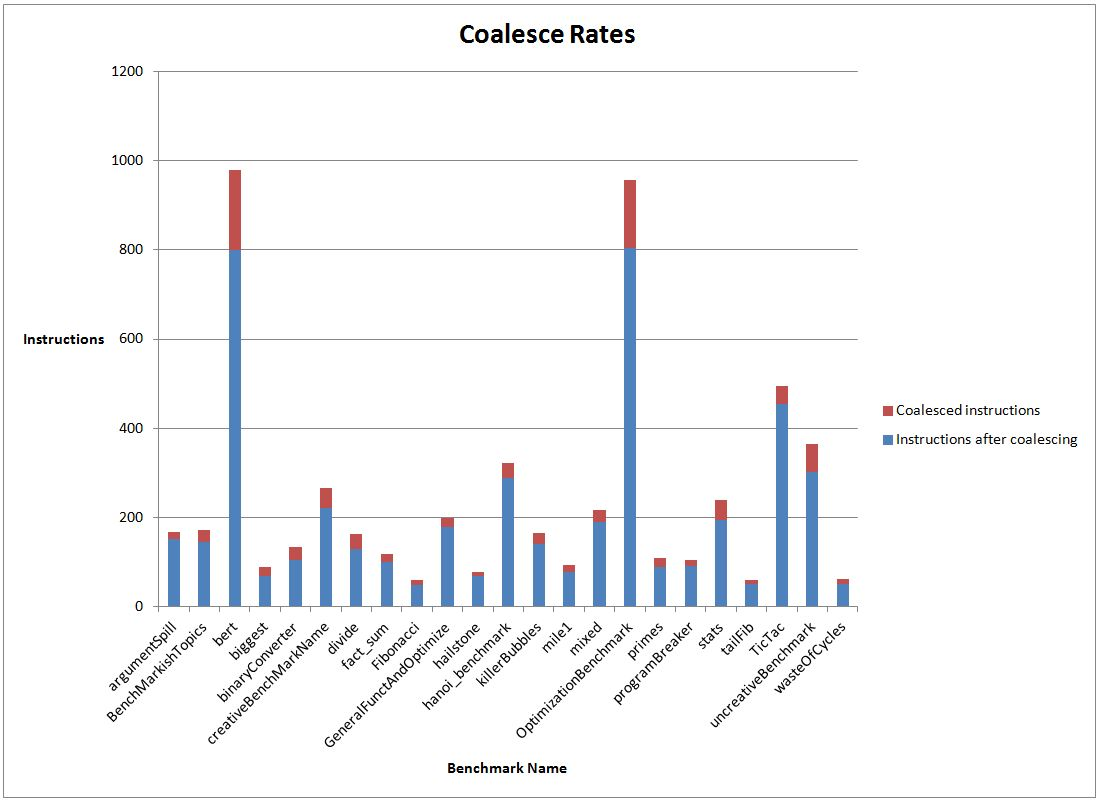
\includegraphics[width=\textwidth]{coalesce_rates.png}
   \caption{Coalesce rates}
   \label{fig:coalesceRates}
\end{figure}

\subsection{Runtime Improvements}
The runtimes in Figure~\ref{fig:indivOpt} were recorded by compiling and each benchmark for each optimization level.
The GNU time utility was used to run the program and output the user time of the program.

Each colored column represents runtime achieved with a particular optimization enabled.
The {\tt -noopt} series indicates benchmark runtimes for the compiler's initial condition - that is, before we began our project.
The {\tt -branchopt} series corresponds to runtimes observed after our branch overhead optimization was implemented.
The {\tt -finline}, {\tt -deadcode}, {\tt -tailcall}, and {\tt -irc} series correspond to function inlining, dead code removal, tail call elimination, and Iterated Register Coalescing, respectively, and were recorded with branch overhead optimization also enabled.
Finally, the {\tt -allopt} series gives benchmark runtimes with all optimizations enabled.

\begin{figure}[H]
   \centering
      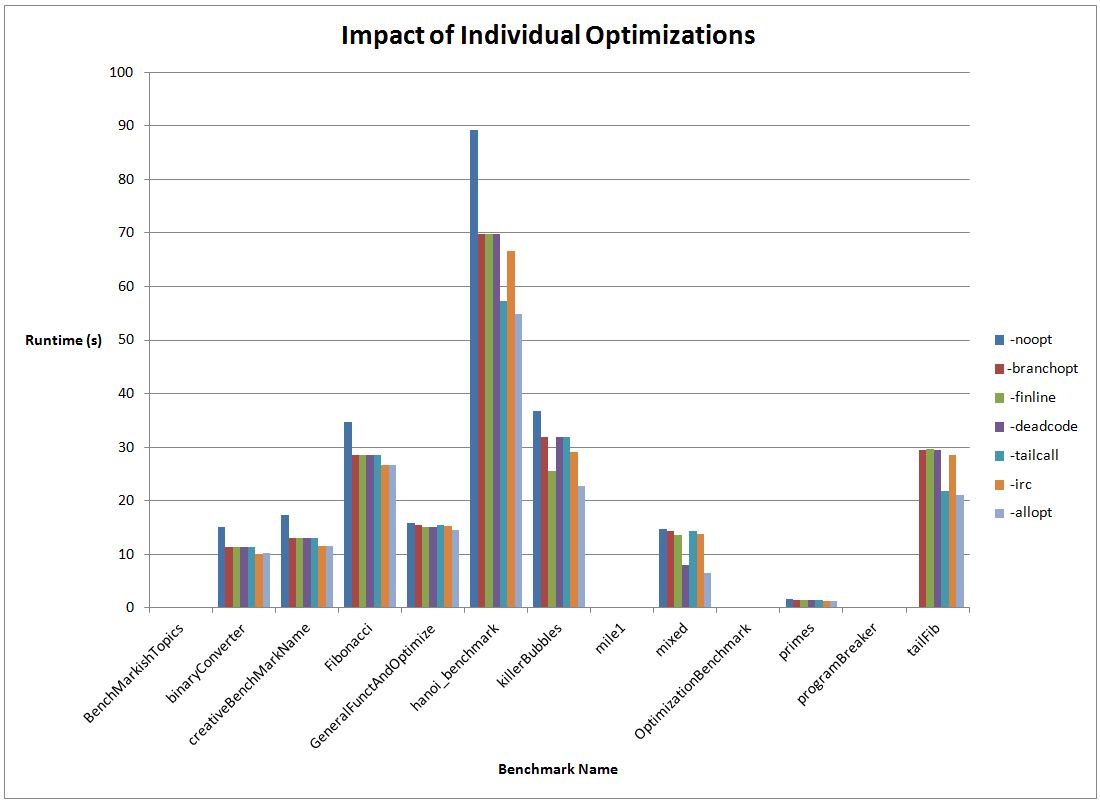
\includegraphics[width=\textwidth]{indiv_opt.png}
   \caption{Impact of Individual Optimizations}
   \label{fig:indivOpt}
\end{figure}

The benchmark programs shown in this graph do not constitute the complete set of benchmarks we used for testing.
Some benchmarks executed so quickly that their runtimes fell below time's minimum resolution.
Since these benchmarks’ runtimes were recorded as 0 for all optimization levels, we decided that they did not provide useful data, and consequently chose to omit most of them.
BenchMarkishTopics is one of these benchmarks, and was included primarily for the sake of completeness.
The time utility did record non-zero runtimes for mile1, OptimizationBenchmark, and programBreaker, but their runtimes are so small that they do not appear on our graph's scale.

It is also important to note that, since the tailFib benchmark was introduced while our project was in progress, we have no runtime data from the compiler's initial state for this benchmark.

\subsection{Comparison to GCC}
The GCC runtimes in Figure~\ref{fig:evilVsGcc} were recorded using the same method that was used to record the EVIL runtimes.
However, since GCC does not compile EVIL code, the EVIL benchmarks were first converted to equivalent C programs, usually with minimal effort.
All runtimes were recorded on the same SPARC machine.

\begin{figure}[H]
   \centering
      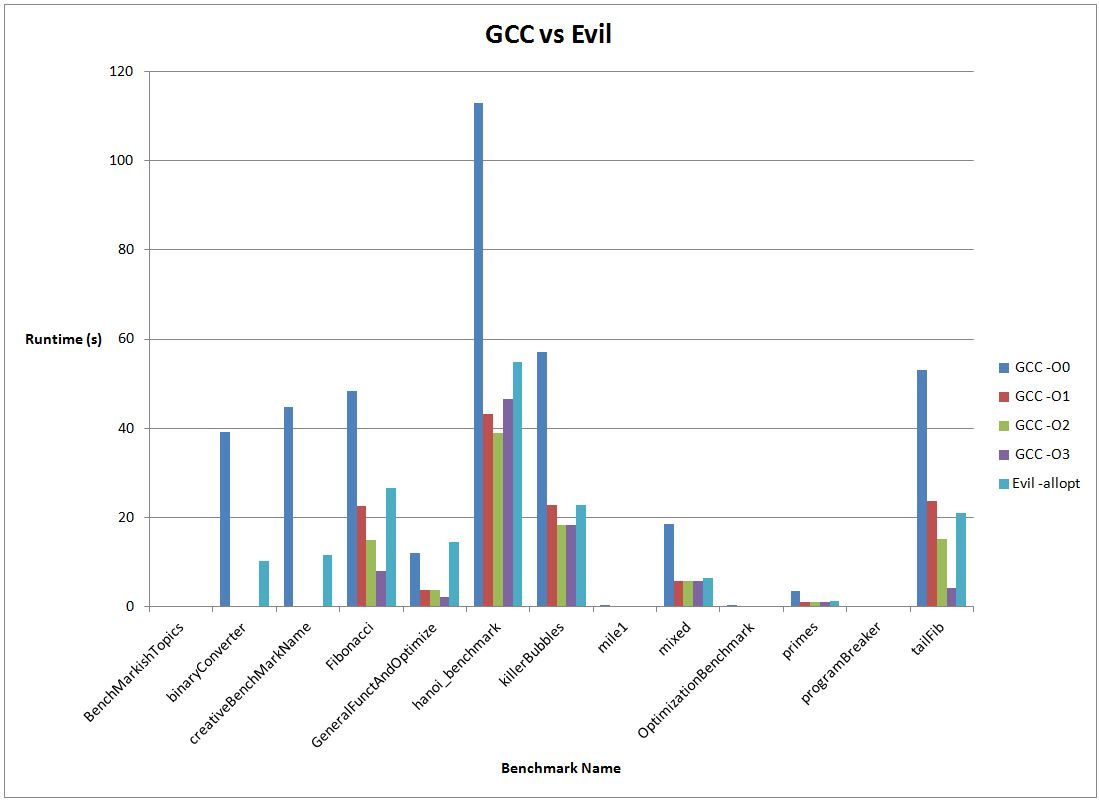
\includegraphics[width=\textwidth]{evil_vs_gcc.png}
   \caption{GCC vs. Evil}
   \label{fig:evilVsGcc}
\end{figure}

As in the previous section, note that most benchmarks with runtimes below time's minimum resolution have been omitted from this figure.

\section{Conclusion}
We learned two main lessons from our experiences during this project.
First, we observed that compiler optimizations are not universally effective.
Instead, their impact depends heavily on the nature of the program being compiled.
Some of our benchmark programs benefited greatly from optimizations that had virtually no effect on other benchmarks.
This demonstrates that a compiler cannot produce consistently optimized code unless it supports a variety of optimizations.

We also gained a new appreciation for the complexity and difficulty of compiler optimization as a whole.
Although the runtime improvements we achieved are noticeable, they are still only small fractions of the benchmarks' total runtimes in almost every case.
Additionally, the optimizations we performed are certainly not cutting-edge and are implemented in every modern compiler.
Through this project, we saw firsthand that compiler optimization is an extremely challenging field, one that demands great effort to achieve comparatively minor results.

\newpage
\bibliographystyle{IEEEannot}
\bibliography{paper}
\end{document}
